\section{Text Quality}
\label{sec:textquality}

When first approaching the topic of measuring the quality
of contributions made by users, our thinking (perhaps shaped
by some of the public discussion surrounding
contributions~\cite{Swartz2006})
focused on the text being added by users.
The basic assumption of a reputation system is that past performance
is a reliable indicator of future performance, so we were
asking the question ``Does text added by some users \intro{survive}
longer than text by other users?''
Note that there are other possible measures of quality, for example:
what size is the contribution; what is the reading level of the
text\cite{Flesch1948,Gunning1952};
how good is the grammar; and does the text seem to be related to
the topic of the article~\cite{Itakura2009}.
We decided not to tackle these kinds of quality measures, both for
the difficulty of natural language processing and because such
methods would require significant work for each language we wanted
to support.
Measuring survival has the advantage that it is relatively cheap to
compute and works the same way across most languages.

To calculate how long a piece of text survives,
we need to track the authorship of
units of text\footnote{For the WikiTrust project, we opted to
use a granularity of words to reduce computational requirements.},
and then compute authorship again in later
versions of the article to find those words with an
authorship dating back to the revision we are trying
to determine the quality of.

In Chapter~\ref{ch:diff}, we describe how to track text authorship
for the text in an article $\article{} \in \articles$.
Just tracking authorship is not enough for tracking survival, since
we need to know what specific revision a word came from.
Let us define another recursive relation, like the definition
for $\txtauthor{}$ in Definition~\ref{def:txtauthor},
which defines the revision where a word was first introduced.
For a word $w_j \in \words{\version{i}}$, we define:
\begin{equation*}
\txtsrcrev{\version{i}, j} =
    \begin{cases}
        \txtsrcrev{\version{k}, s}, & \text{ if }
        \match{\version{i}, j, \prevrevs{\version{i}}} = (\version{k}, s) \\
        i, & \text{ if there is no best match text. } \\
    \end{cases}
\end{equation*}
Now we can define the text survival of words to be the number of
words introduced in \version{m} still present in \version{n}:
\begin{equation}
\tsurv{\article{}}{m,n} = \left| \left\{ j \colon
    \exists j \in \mathbb{Z} . ( \txtsrcrev{\version{n},j} = m ) \right\} \right| \\
\label{eq:tsurv}
\end{equation}

\subsection{Text Decay Quality}

In the abstract, our goal is to define some metric that we can compute for
revisions that quantifies some estimate of the \intro{quality} of the
revision.
There are many possible ways to define quality measures, which is the
subject of research on vandalism detection (see
Section~\ref{sec:vandalism-related} for background on that topic).
As an example, a simple quality measure would be the heuristic that
inappropriate words added as part of an edit would indicate that the revision
is of poor quality.

For the purpose of building a reputation system, we want a measure
that provides some insight into the community perception of the
quality of the edit.
Having defined the notion of text survival, a very simple quality measure
could be ``What fraction of the text added in a revision survives
ten revisions later?''
We discuss some variations of these quality measures in
Chapter~\ref{ch:contrib}, but present one novel quality measure here.

\begin{figure}[htbp]
\centering
\framebox{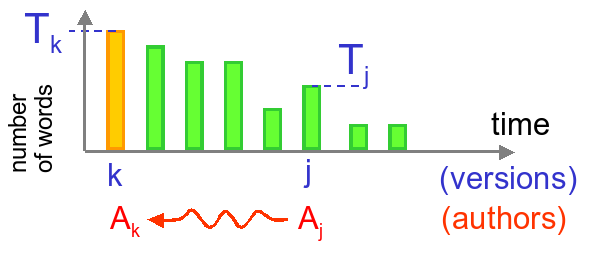
\includegraphics[width=0.9\textwidth]{part-F70-editquality/textcontr-2}}
\caption{A graphical depiction of how a text contribution survives
	through future revisions.
        An author, \editor{k}, adds
    $T_k = \tsurv{}{k,k}$ words in revision \version{k}.  In subsequent
    revisions, some of those words are deleted and partially restored.
    We say that a later author, \editor{j}, implicitly \intro{judges}
    author \editor{k} by choosing how many of \editor{k}'s words
    to keep or delete or restore; $T_j = \tsurv{}{k,j}$ is the number of words
    that were introduced in \version{k} still present or
    \intro{live}, in \version{j}.
}
\label{fig:textsurvival} 
\end{figure}


In trying to understand how text contributions evolve, we decided
to limit our exploration to what happens to the text over the
following ten revisions.
Many contributions follow the simplest model: they are either
removed completely right away (a revert), or they are perfectly
preserved for the following ten revisions.
Some contributions, however, are only partially preserved, and
might even be partially restored as part of their evolution.
Figure~\ref{fig:textsurvival} gives a pictorial representation
of how some text introduced at revision \version{k} might
evolve over the next seven revisions; in this example, the
figure shows that some text was restored in revision \version{j}.
We say that author $A_j$ \intro{judges} the work of author
$A_k$ by deciding how much text to preserve, delete, or restore.
If author $A_j$ works on a different part of the article, she
is still implicitly deciding that the current revision of
$A_k$'s work is okay.\footnote{Some better model of
user attention would be useful for tempering the amount
of judgement we infer from
$A_k$ when they are focused elsewhere in the article.}

Measuring the fraction of text introduced in
revision \version{k} that survives to revision \version{j}
(\ie computing $\tsurv{}{k,j} / \tsurv{}{k,k}$)
gives useful information, but what if \version{j} happens to be
a vandal that blanks the page?
One idea would be to average the text survival over the next
several revisions (an idea explored in Chapter~\ref{ch:contrib}),
but we were struck by the observation that after some initial
churning, text seems to stabilize and then only slowly change
as time progresses.
We propose that one way to model this evolution of text over time
is as a geometric sequence with a common ratio between zero and one;
see Figure~\ref{fig:textlongevity} for how such a sequence could
approximate the text survival over several revisions.
The intuition behind a geometric model is that if an edit is
``bad,'' then most of the text will be removed right away.
As time passes, the size of the edits decreases and
the text tends to stabilize into a form
that people can agree on until it eventually no longer changes.


\begin{figure}[tbph]
\centering
\framebox{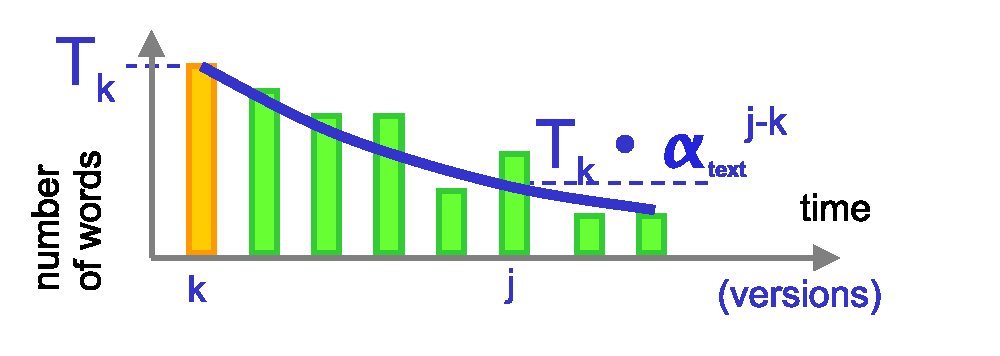
\includegraphics[width=0.9\textwidth]{part-F70-editquality/text-longevity}}
\caption{
    \mynote{Redo picture to change alpha to proper symbol.}
    To calculate the \intro{text longevity} of the contribution
    of $T_k$ words, we model the text survival as a geometric curve
    and compute a single number that describes how the text evolves
    over several revisions.}
\label{fig:textlongevity}
\end{figure}

\begin{figure}[tbph]
\centering
\framebox{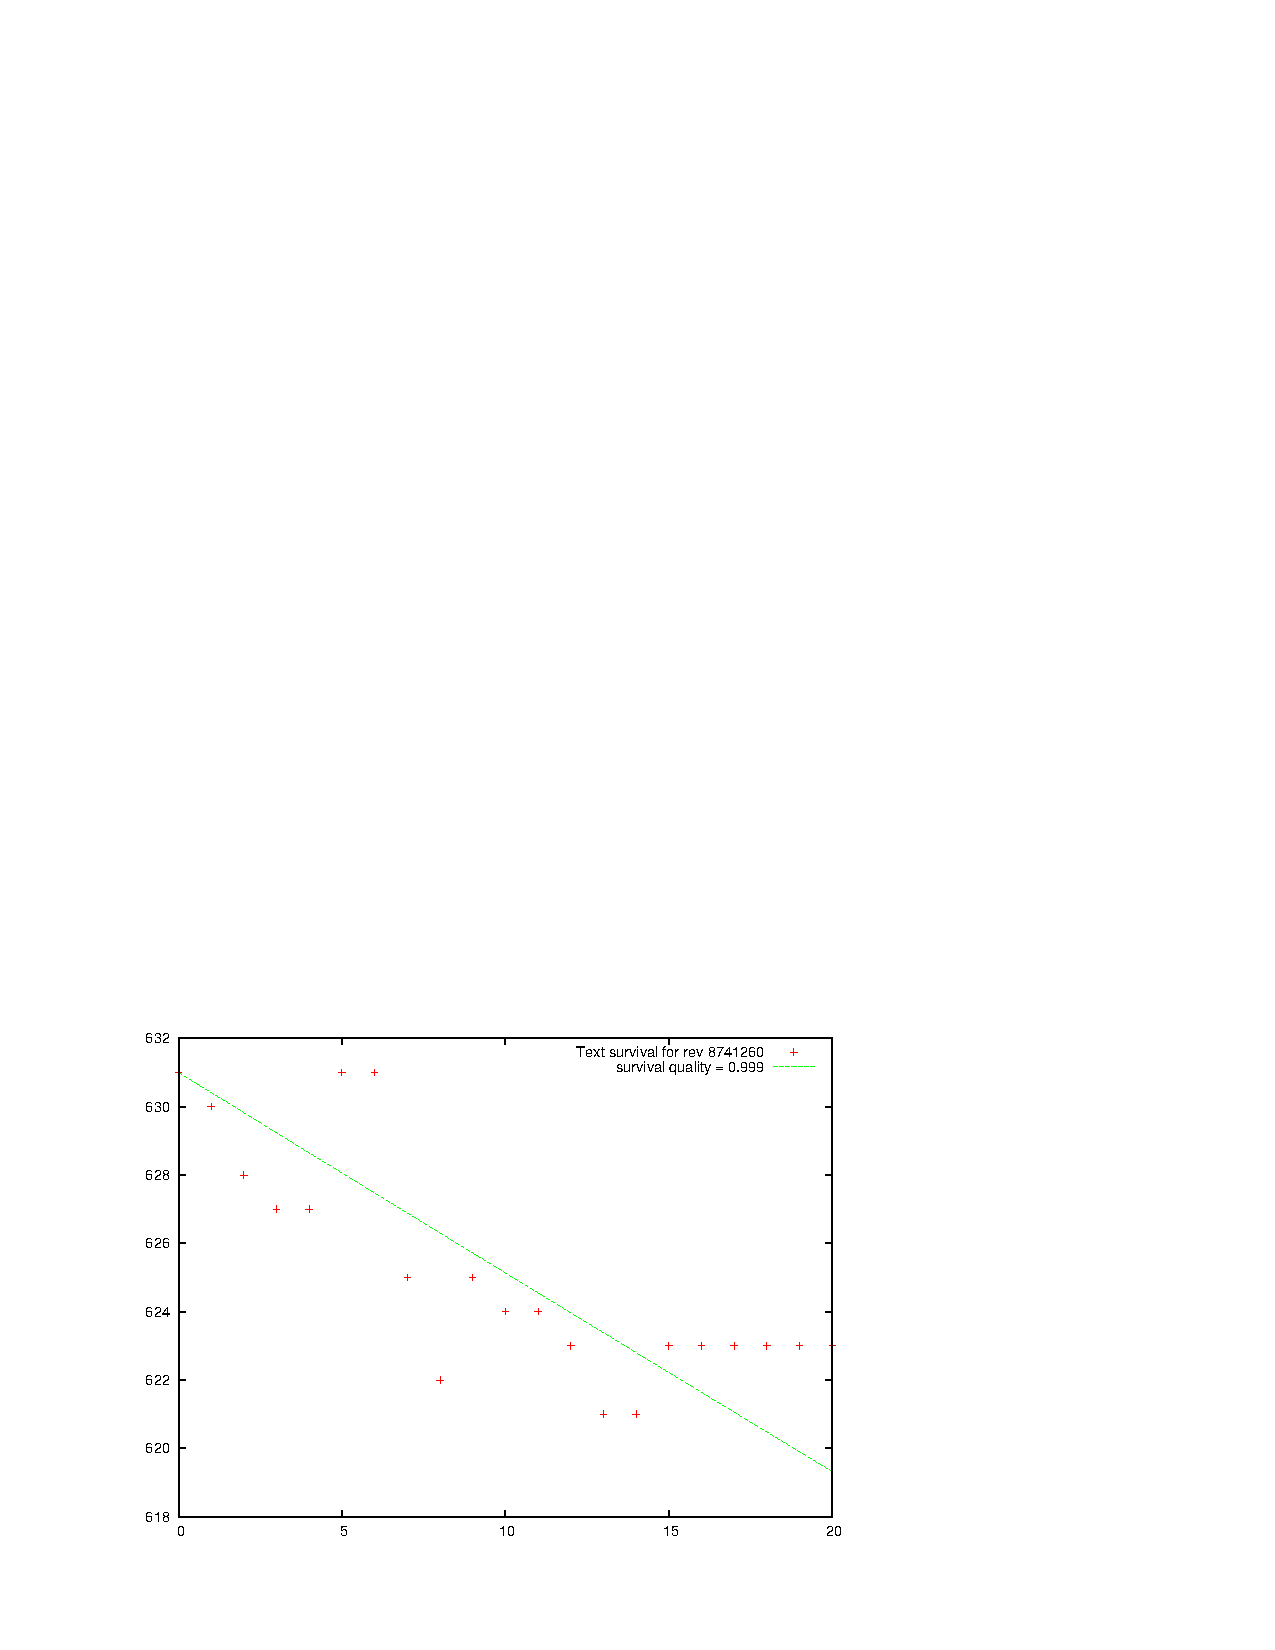
\includegraphics[width=0.95\textwidth]{part-F70-editquality/graph-TS-SantaCruzBeachBoardwalk}}
\caption{The text survival graph for the text initially contributed
	as part of the article \textit{Santa Cruz Beach Boardwalk}.
	The majority of the editing to the contributed text happens
	in the next few revisions, before the text stabilizes.
	The graph also shows the text survival quality
	computed based on 20~revisions.
	}
\label{fig:ts-SantaCruzBeachBoardwalk}
\end{figure}

To measure the overall quality of a single text contribution
made in revision \version{k}, we need to compute the common ratio
that best describes the sequence of $n$ text survival values,
\tsurv{}{k,j}, after \version{k}, where $k < j \le k+n$.
Let us call this common ratio the \intro{text decay quality},
\quality{tdecay}{n}{k}.
To compute \quality{tdecay}{n}{k}, we want to solve the following equation:
\begin{align*}
    \sum_{i=0}^n \tsurv{}{k,k+i} = {} & \tsurv{}{k,k} + \quality{tdecay}{n}{k} \cdot \tsurv{}{k,k+1} \\
    & + (\quality{tdecay}{n}{k})^2 \cdot \tsurv{}{k,k+2} + \ldots \\
    & + (\quality{tdecay}{n}{k})^n \cdot \tsurv{}{k,k+n} \\
    = {} & \tsurv{}{k,k} \cdot \sum_{i=0}^n (\quality{tdecay}{n}{k})^i \\
    = {} & \tsurv{}{k,k} \cdot \frac{1 - (\quality{tdecay}{n}{k})^{n+1}}{1 - \quality{tdecay}{n}{k}} \\
\end{align*}

To solve this for \quality{tdecay}{}{k}, we can use Newton's method
to solve for the zero of the related function:
\begin{equation*}
  f(\alpha) =
        - (1 - \alpha^{n+1}) \cdot \tsurv{}{k,k}
        + (1 - \alpha) \cdot \sum_{i=0}^n \tsurv{}{k,k+i}
\end{equation*}
where $\alpha = \quality{tdecay}{}{k}$.
Newton's method involves making repeated estimations of the form
\begin{equation*}
  \alpha_{j+1} = \alpha_j - \frac{f(\alpha_j)}{f'(\alpha_j)}
\end{equation*}
which we initiate with $\alpha_0 = 0$.
For efficiency reasons, we limit the number of iterations taken
to a small number (five in our live system)
since we are only estimating the quality, and high precision
is not very useful.

The beauty of this quality measure is that it varies between
zero for text that is immediately deleted, and one, for text
that is completely preserved.
Values in between the two extremes reflect the fact that there
was some debate among the community about what text to preserve
in the article.
Figure~\ref{fig:ts-SantaCruzBeachBoardwalk} shows the text survival
graph of the initial contribution to that article and of how it varies
over the next twenty filtered revisions.
The figure also shows the curve representing the decay quality,
calculated with a twenty-iteration Newton's method over the entire
twenty-one revision sequence.

\mynote{TODO: Still running author tracking on GWB page, redherring screen 2,
Sat, 5-Feb.}

